\section{Constructing the Training Target}

\label{sec:fokker_planck}

In the previous section, we constructed flow and diffusion models where we obtain trajectories $(X_t)_{0\leq t\leq 1}$ by simulating the ODE/SDE

在前一节中,我们构建了流模型和扩散模型,通过模拟常微分方程/随机微分方程来获得轨迹 $(X_t)_{0\leq t\leq 1}$
\begin{align}
\label{e:sde_generative_model_restated_section_3}
 X_0\sim&\pinit,\quad \dd X_t = u_t^\theta(X_t)\dd t& \text{(Flow model)}\\
 X_0\sim&\pinit,\quad \dd X_t = u_t^\theta(X_t)\dd t + \sigma_t\dd W_t& \text{(Diffusion model)}
\end{align}
where $u_t^\theta$ is a neural network and $\sigma_t$ is a fixed diffusion coefficient. Naturally, if we just randomly initialize the parameters $\theta$ of our neural network $u_t^\theta$, simulating the ODE/SDE will just produce nonsense. As always in machine learning, we need to train the neural network. We accomplish this by minimizing a loss function $\mathcal{L}(\theta)$, such as the \themebf{mean-squared error}

其中 $u_t^\theta$ 是一个神经网络,$\sigma_t$ 是固定的扩散系数。显然,如果我们只是随机初始化神经网络 $u_t^\theta$ 的参数 $\theta$,模拟 ODE/SDE 只会产生无意义的结果。正如机器学习中的惯例,我们需要训练神经网络。我们通过最小化损失函数 $\mathcal{L}(\theta)$ 来实现这一点,比如 \themebf{均方误差}
\begin{align*}
    \mathcal{L}(\theta) = \lVert u_t^\theta(x)-\underbrace{\uref_t(x)}_{\text{training target}}\rVert^2 ,
\end{align*}
where $\uref_t(x)$ is the \themebf{training target} that we would like to approximate. To derive a training algorithm, we proceed in two steps: In this chapter, our goal is to \textbf{find an equation for the training target $\uref_t$}. In the next chapter, we will describe a training algorithm that approximates the training target $\uref_t$. Naturally, like the neural network $u_t^\theta$, the training target should itself be a vector field $\uref_t:\mathbb{R}^d\times[0,1]\to\mathbb{R}^d$. Further, $\uref_t$ should do what we want $u_t^\theta$ to do: convert noise into data. \textbf{Therefore, the goal of this chapter is to derive a formula for the training target $u_t^\text{ref}$ such that the corresponding ODE/SDE converts $\pinit$ into $\pdata$}. Along the way we will encounter two fundamental results from physics and stochastic calculus: the \themebf{continuity equation} and the \themebf{Fokker-Planck equation}. As before, we will first describe the key ideas for ODEs before generalizing them to SDEs.

其中 $\uref_t(x)$ 是我们希望逼近的 \themebf{训练目标}。为了推导训练算法,我们分两步进行:在本章中,我们的目标是 \textbf{找到训练目标 $\uref_t$ 的方程}。在下一章中,我们将描述一个逼近训练目标 $\uref_t$ 的训练算法。显然,与神经网络 $u_t^\theta$ 一样,训练目标本身应该是一个向量场 $\uref_t:\mathbb{R}^d\times[0,1]\to\mathbb{R}^d$。此外,$\uref_t$ 应该完成我们希望 $u_t^\theta$ 完成的任务:将噪声转换为数据。\textbf{因此,本章的目标是推导训练目标 $u_t^\text{ref}$ 的公式,使得相应的 ODE/SDE 将 $\pinit$ 转换为 $\pdata$}。在此过程中,我们将遇到物理学和随机演算中的两个基本结果:\themebf{连续性方程} 和 \themebf{福克-普朗克方程}。如前所述,我们将首先描述 ODE 的关键思想,然后将其推广到 SDE。

\begin{remarkbox}
There are a number of different approaches to deriving a training target for flow and diffusion models. The approach we present here is both the most general and arguably most simple and is in line with recent state-of-the-art models. However, it might well differ from other, older presentations of diffusion models you have seen. Later, we will discuss  alternative formulations.

对于流模型和扩散模型的训练目标,存在多种不同的推导方法。我们在此介绍的方法既是最通用的,也可以说是最简单的,并且与最近的最先进模型保持一致。然而,它可能与您之前见过的其他较早的扩散模型表述有所不同。稍后,我们将讨论其他的公式化方法。
% \cref{subsec:guide_to_flow_matching_literature}.
\end{remarkbox}

\begin{figure}[h!]
    \centering
    \begin{tabular}{ccc}
         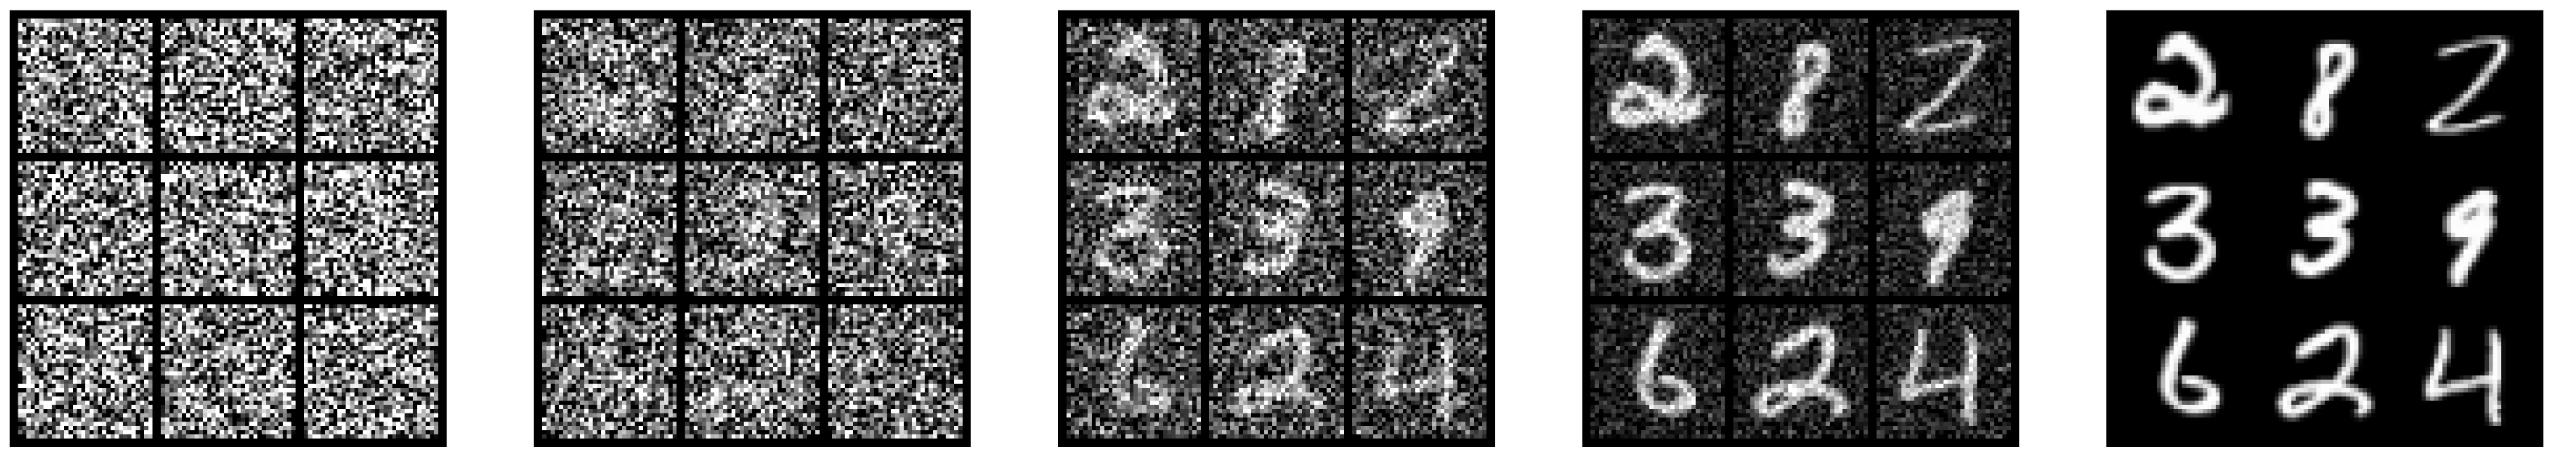
\includegraphics[width=\textwidth]{figures/noised_mnist_reversed.png} &
    \end{tabular}
    \caption{\label{fig:noising_image} Gradual interpolation from noise to data via  a Gaussian conditional probability path for a collection of images.\\通过高斯条件概率路径从噪声到数据的一组图像的渐进插值。}
\end{figure}

\subsection{Conditional and Marginal Probability Path}

The first step of constructing the training target $\uref_t$ is by specifying a \themebf{probability path}. Intuitively, a probability path specifies a gradual interpolation between noise $\pinit$ and data $\pdata$ (see \cref{fig:noising_image}). We explain the construction in this section. In the following, for a data point $z\in\mathbb{R}^d$, we denote with $\delta_{z}$ the \themebf{Dirac delta} ``distribution''. This is the simplest distribution that one can imagine: sampling from $\delta_{z}$ always returns $z$ (i.e. it is deterministic). A \themebf{conditional (interpolating) probability path} is a set of distribution $p_t(x|z)$ over $\mathbb{R}^d$ such that:

构建训练目标 $\uref_t$ 的第一步是指定一个 \themebf{概率路径}。直观地说,概率路径指定了噪声 $\pinit$ 和数据 $\pdata$ 之间的渐进插值(见\cref{fig:noising_image})。我们在本节中解释这种构建方法。在下文中,对于数据点 $z\in\mathbb{R}^d$,我们用 $\delta_{z}$ 表示 \themebf{狄拉克delta} "分布"。这是人们可以想象的最简单的分布:从 $\delta_{z}$ 采样总是返回 $z$(即它是确定性的)。\themebf{条件(插值)概率路径} 是在 $\mathbb{R}^d$ 上的一组分布 $p_t(x|z)$,满足:
\begin{align}
    % p_t(\cdot|z) \text{ distribution over }\R^d \quad (0\leq t\leq 1)\\
\label{eq:interpolating_condition_conditional_path}
    p_0(\cdot|z)=\pinit, \quad p_1(\cdot|z)=\delta_{z}\quad \text{ for all }z\in\R^d.
\end{align}
In other words, a conditional probability path gradually converts a \themeit{single} data point into the distribution $\pinit$ (see e.g. \cref{fig:noising_image}). You can think of a probability path as a trajectory in the space of distributions. Every conditional probability path $p_t(x|z)$ induces a \themebf{marginal probability path} $p_t(x)$ defined as the distribution that we obtain by first sampling a data point $z\sim \pdata$ from the data distribution and then sampling from $p_t(\cdot|z)$:

换句话说,条件概率路径逐渐将 \themeit{单个} 数据点转换为分布 $\pinit$(例如见\cref{fig:noising_image})。您可以将概率路径视为分布空间中的轨迹。每个条件概率路径 $p_t(x|z)$ 诱导一个 \themebf{边际概率路径} $p_t(x)$,定义为我们首先从数据分布中采样数据点 $z\sim \pdata$,然后从 $p_t(\cdot|z)$ 中采样所得到的分布:
\begin{align}
    \label{eq:marginal_prob_path}
    z&\sim\pdata, \quad x\sim p_t(\cdot|z)\quad \Rightarrow x\sim p_t &&\blacktriangleright\,\,\text{sampling from marginal path}\\
    p_t(x) &= \int p_t(x|\dap) \pdata (z) \dd z &&\blacktriangleright\,\,\text{density of marginal path}
\end{align}
Note that we know how to sample from $p_t$ but we don't know the density values $p_t(x)$ as the integral is intractable. Check for yourself that because of the conditions on $p_t(\cdot|z)$ in \cref{eq:interpolating_condition_conditional_path}, the marginal probability path $p_t$ interpolates between $\pinit$ and $\pdata$:

注意,我们知道如何从 $p_t$ 中采样,但由于积分是不可处理的,我们不知道密度值 $p_t(x)$。您可以自己验证,由于 \cref{eq:interpolating_condition_conditional_path} 中对 $p_t(\cdot|z)$ 的条件,边际概率路径 $p_t$ 在 $\pinit$ 和 $\pdata$ 之间插值:
\begin{align}
\label{eq:noise_interpolation}
p_0 =\pinit\quad\text{and}\quad p_1=\pdata.\quad\quad\quad\quad \blacktriangleright\,\,\text{noise-data interpolation}
\end{align}
\begin{figure}[!t]
    \centering
    \begin{tabular}{ccc}
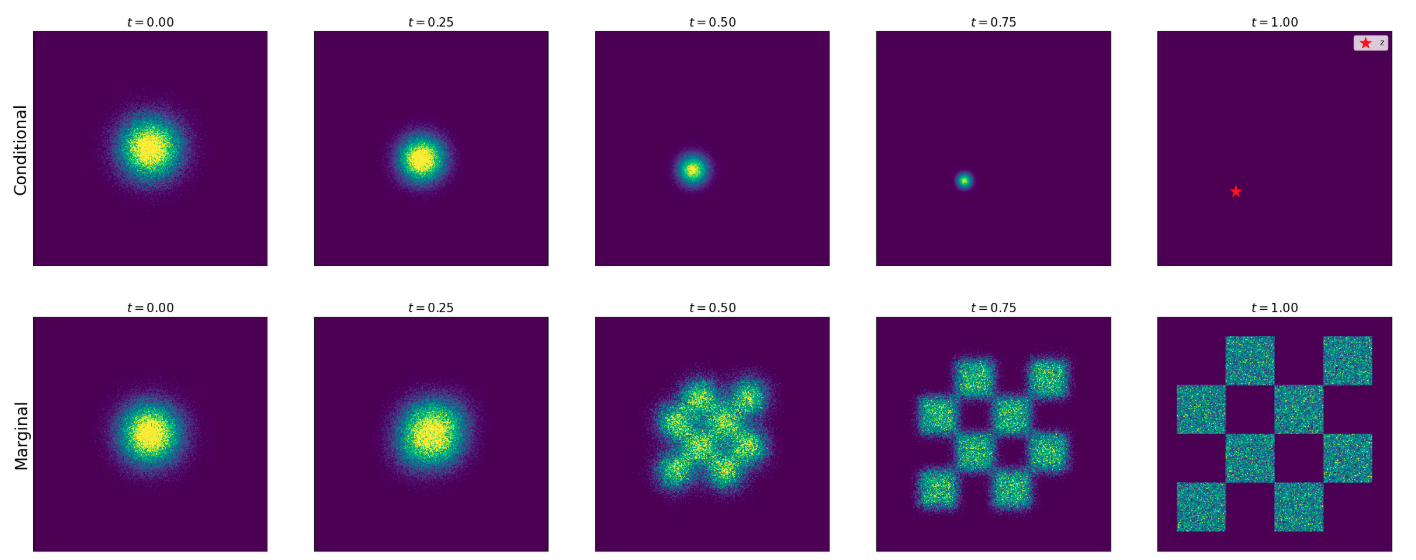
\includegraphics[width=\textwidth]{figures/conditional_vs_marginal.png} &
         % 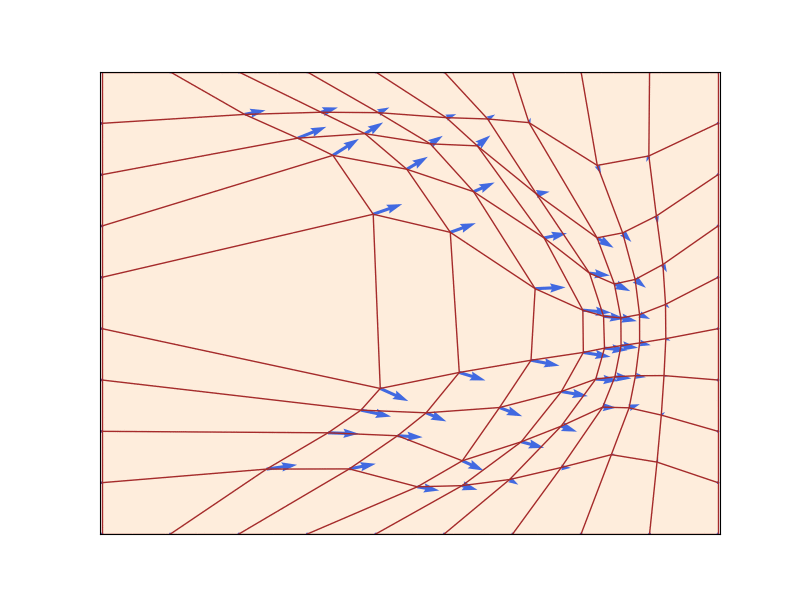
\includegraphics[width=0.3\textwidth]{fm_guide_assets/flow_16.png} 
    \end{tabular}
\caption{\label{fig:cond_marginal_path_histograms}Illustration of a conditional (top) and marginal (bottom) probability path. Here, we plot a Gaussian probability path with $\alpha_t=t,\beta_t=1-t$. The conditional probability path interpolates a Gaussian $\pinit=\mathcal{N}(0,I_d)$ and $\pdata=\delta_{z}$ for single data point $z$. The marginal probability path interpolates a Gaussian and a data distribution $\pdata$ (Here, $\pdata$ is a toy distribution in dimension $d=2$ represented by a chess board pattern.)\\条件(上)和边际(下)概率路径的图解。这里,我们绘制了高斯概率路径,其中 $\alpha_t=t,\beta_t=1-t$。条件概率路径在高斯分布 $\pinit=\mathcal{N}(0,I_d)$ 和单个数据点 $z$ 的 $\pdata=\delta_{z}$ 之间进行插值。边际概率路径在高斯分布和数据分布 $\pdata$ 之间进行插值(这里,$\pdata$ 是维度 $d=2$ 中由棋盘图案表示的玩具分布)。}
\end{figure}
% Note our goal in \cref{e:end_points_match} doesn't say anything about how $p_t^\theta$ should look like for intermediate time points $0<t<1$. Therefore, there is more degrees of freedom that we are allowed to choose.\footnote{It is also possible to optimize over all possible $p_t^\theta$. An example is Neural ODEs (see \cref{subsec:neural_odes}) or Schrödinger Bridges \citep{shi2024diffusion}. However, these methods usually don't scale well to large high-dimensional data such as images, videos, or molecules.}We do so by specifying an \themebf{(interpolating) probability path} $(p_t)_{0\leq t\leq 1}$ given by:
% \begin{align}
%     p_t \text{ distribution over }\R^d \quad (0\leq t\leq 1)\\
%     \label{eq:interpolating_condition}
%     p_0=\pinit, \quad p_1=\pdata
% \end{align}
% Intuitively, an interpolating probability path starts at the distribution $\pinit$ and ends at distribution $\pdata$. With this, we can say that we want $p_t^\theta$ to match $p_t$ along the entire trajectory:
% \begin{align}
%     \label{eq:prob_path_matching}
%     \textbf{Matching probability paths: }p_t^\theta = p_t \quad \text{ for all }0\leq t \leq 1
% \end{align}
% Therefore, we guide the trajectory for all $0\leq t\leq 1$. This is a stronger but sufficient requirement for final distributions to match (see \cref{e:end_points_match}). However, it is intuitive why this might be beneficial: we give "feedback" along the whole trajectory instead of only at the end. The most important reason is however: There exists a nice mathematical equation to ensure that \cref{eq:prob_path_matching} holds, specifically the famous \emph{Fokker-Planck Equation} that we will explain in the next section. In this section, it remains to explain how one can construct interpolating probability paths.

% \paragraph{Conditional probability path.} Let us consider the most simple data distribution that one can imagine: a single data point. In other words, $\pdata=\delta_{\dap}$ where $z\in\mathbb{R}^d$ is a fixed point. The notation $\delta_{\dap}$ refers to the \themebf{Dirac delta} distribution.  Sampling from $\pdata=\delta_{\dap}$ will always return the same point $\dap$. It is therefore a rather trivial distribution. Let us try to convert $\delta_z$ into the distribution $\pinit$. We do this via \themebf{conditional (interpolating) probability path} $p_t(x|z)$ defined via
% \begin{align}
%     p_t(\cdot|z) \text{ distribution over }\R^d \quad (0\leq t\leq 1)\\
% \label{eq:interpolating_condition_conditional_path}
%     p_0(\cdot|z)=\pinit, \quad p_1(\cdot|z)=\delta_{z}\quad \text{ for all }z\in\R^d
% \end{align}
% In other words, a conditional probability path gradually converts a single data point into the distribution $p_0=\pinit$. Let's examine several examples of conditional probability paths.

\begin{examplebox}[Gaussian Conditional Probability Path]
\label{example:gaussian_path}
    One particularly popular probability path is the \themebf{Gaussian probability path}. This is the \textbf{probability path used by denoising diffusion models}. Let $\alpha_t,\beta_t$ be \themebf{noise schedulers}: two continuously differentiable, monotonic functions with $\alpha_0=\beta_1=0$ and $\alpha_1=\beta_0=1$. We then define the conditional probability path

    一个特别流行的概率路径是 \themebf{高斯概率路径}。这是 \textbf{去噪扩散模型使用的概率路径}。设 $\alpha_t,\beta_t$ 为 \themebf{噪声调度器}:两个连续可微的单调函数,满足 $\alpha_0=\beta_1=0$ 和 $\alpha_1=\beta_0=1$。然后我们定义条件概率路径
\begin{align}
\label{eq:gaussian_conditional_probability_paths}
p_t(\cdot|\dap) &= \mathcal{N}(\alpha_t \dap,\beta_t^2 I_d)
& \blacktriangleright \,\, \text{Gaussian conditional path/高斯概率路径}
\end{align}
which, by the conditions we imposed on $\alpha_t$ and $\beta_t$, fulfills

根据我们对 $\alpha_t$ 和 $\beta_t$ 施加的条件,这满足
\begin{align*}
    p_0(\cdot|\dap) &= \mathcal{N}(\alpha_0 \dap,\beta_0^2 I_d) = \mathcal{N}(0,I_d),\quad \text{and}\quad
p_1(\cdot|\dap) = \mathcal{N}(\alpha_1 \dap,\beta_1^2 I_d) = \delta_{\dap},
\end{align*}
where we have used the fact that a normal distribution with zero variance and mean $\dap$ is just $\delta_{\dap}$. Therefore, this choice of $p_t(x|\dap)$ fulfills \cref{eq:interpolating_condition_conditional_path} for $\pinit=\mathcal{N}(0,I_d)$ and is therefore a valid conditional interpolating path. The Gaussian conditional probability path has several useful properties which makes it especially amenable to our goals, and because of this we will use it as our prototypical example of a conditional probability path for the rest of the section. In \cref{fig:noising_image}, we illustrate its application to an image. We can express sampling from the marginal path $p_t$ as:

其中我们利用了方差为零、均值为 $\dap$ 的正态分布就是 $\delta_{\dap}$ 这一事实。因此,对于 $\pinit=\mathcal{N}(0,I_d)$,这种 $p_t(x|\dap)$ 的选择满足 \cref{eq:interpolating_condition_conditional_path},因此是一个有效的条件插值路径。高斯条件概率路径具有几个有用的性质,使其特别适合我们的目标,因此我们将在本节的其余部分使用它作为条件概率路径的原型示例。在 \cref{fig:noising_image} 中,我们展示了它在图像上的应用。我们可以将从边际路径 $p_t$ 采样表示为: 
\begin{align}
    \label{eq:gaussian_prob_path_sampling}
    z\sim&\pdata,\,\epsilon\sim\pinit = \mathcal{N}(0,I_d) \,\Rightarrow\, x=\alpha_tz+\beta_t \epsilon\sim p_t \quad &\blacktriangleright \,\,\text{sampling from marginal Gaussian path/从边际高斯路径采样}
\end{align}
Intuitively, the above procedure adds more noise for lower $t$ until time $t=0$, at which point there is only noise. In \cref{fig:cond_marginal_path_histograms}, we plot an example of such an interpolating path between Gaussian noise and a simple data distribution.

直观地说,上述过程为较小的 $t$ 添加更多噪声,直到时间 $t=0$,此时只有噪声。在 \cref{fig:cond_marginal_path_histograms} 中,我们绘制了高斯噪声和简单数据分布之间这种插值路径的一个示例。
\end{examplebox}

% \paragraph{Marginal probability path.}
% Let now be $\pdata$ be arbitrary again. How can we convert $\pdata$ into $\pinit$? As we just learnt, we can do it for a fixed data point $z\in \mathbb{R}^d$ with a conditional interpolating path $p_t(\cdot|z)$. We can naturally extend this to $\pdata$ via the hierarchical sampling procedure:
% \begin{subequations}
% \label{eq:sampling_procedure_marginal_path}
% \begin{align}
%     &\text{Step 1. Draw random data point from data set: }z\sim \pdata\\
%     &\text{Step 2. Draw sample from conditional interpolating path: }x\sim p_t(\cdot|z)
% \end{align}
% \end{subequations}

% We call the distribution $p_t$ of the resulting sample $x$ the \themebf{marginal (interpolating) probability path}, i.e. $x\sim p_t$. We can express the probability density of $p_t$ via
% \begin{align}
%     \label{eq:marginal_prob_path}
%     p_t(x) = \int p_t(x|\dap) \pdata (z) \dd z
% \end{align}
% i.e. we marginalize over the data distribution. Note that because of the conditions on $p_t(\cdot|z)$ in \cref{eq:interpolating_condition_conditional_path}, the marginal probability path $p_t$ interpolates between $\pinit$ and $\pdata$:
% \begin{align*}
% p_0 = \pinit,\quad p_1=\pdata
% \end{align*}
% You can check this for yourself: If $t=0$, then $p_t(x|z)=\pinit$ regardless of $z$ (see \cref{eq:interpolating_condition_conditional_path}). Therefore, our sample $x$ will always be a sample $\pinit$ regardless of $z$. Therefore, $p_0=\pinit$. For $t=1$, we know by the definition of $\delta_{\dap}$ that $x=z\sim \pdata$. Therefore, $x\sim p_1=\pdata$.

% In other words, we found a gradual way of converting data $\pdata$ into noise $\pinit$. In \ph{INSERT FIGURE}, we plot the marginal probability path of a simple data distribution.
% How would we construct an interpolating probability path? The answer is by choosing a conditional path $p_t(x|\dap)$ and then define
% \begin{align}
%     p_t(x) = \int p_t(x|\dap) \pdata (z) \dd z
% \end{align}
% To differentiate it from $p_t(x|z)$, we call now $p_t(x)$ the \themebf{marginal (interpolating) probability path} (because you obtain it from $p_t(x|z)$ by marginalizing over the data distribution $\pdata$). The above expresses $p_t$ in the form of its probability density as an integral. It might be easier to think about how we would draw samples from the distribution $p_t$. This can be done as follows:
% \begin{align*}
%     &\text{Step 1. Draw random data point from data set: }z\sim \pdata\\
%     &\text{Step 2. Draw sample from conditional interpolating path: }x\sim p_t(\cdot|z)\\
%     \Rightarrow &\text{The resulting sample }x\text{ will have distribution }p_t
% \end{align*}
%This shows that, as desired, $p_t$ interpolates $\pinit$ and $\pdata$ (i.e. \cref{eq:interpolating_condition} is fulfilled).




% \paragraph{Summary.} Let us summarize the results of this section. In order to generate samples from $\pdata$, we choose an conditional interpolating probability path $p_t(x|\daz)$ that converts data into "noise", i.e. that fulfils
% \begin{align*}
%     \textbf{Conditional (interpolating) probability path: } p_0(\cdot|z)=\pinit, p_1(\cdot|z)=\delta_{z}
% \end{align*}
% and construct a diffusion model with neural network $u_t^\theta$
% \begin{align}
% \label{e:sde_generative_model_restated_section_3}
%  \textbf{diffusion model: }X_0\sim&\pinit,\quad \dd X_t = u_t^\theta(X_t)\dd t + \sigma_t\dd W_t
% \end{align}
% Our goal is to train $u_t^\theta$ such that it reverses this noising process, i.e. such that the distribution $p_t^\theta$ of $X_t$ matches the distribution marginalized over data points:
% \begin{align}
% \label{eq:prob_path_matching_summary}
%     \textbf{Matching marginal probability paths: }p_t^\theta = p_t =\int p_t(x|z)\pdata(z)\dd z \quad \text{ for all }0\leq t \leq 1
% \end{align}
% Step-by-step we now made the generative model problem more specific. The problem is that \cref{eq:prob_path_matching_summary} is a condition that is hard to train a machine learning for: remember, we only have access to the neural network $u_t^\theta$ explicitly but we don't really know $p_t^\theta$. Fortunately, there is a famous equation that allows us to simplify it further that we will discuss next.



\subsection{Conditional and Marginal Vector Fields}

We proceed now by constructing a training target $\uref_t$ for a flow model using the recently defined notion of a probability path $p_t$. The idea is to construct $\uref_t$ from simple components that we can derive analytically by hand.

我们现在使用刚刚定义的概率路径 $p_t$ 概念来为流模型构建训练目标 $\uref_t$。其思想是从可以手工解析推导的简单组件构建 $\uref_t$。
\begin{theorem}[Marginalization trick]
\label{thm:marginalization_trick}
For every data point $z\in \mathbb{R}^d$, let $\uref_t(\cdot|z)$ denote a \themebf{conditional vector field}, defined so that the corresponding ODE yields the conditional probability path $p_t(\cdot|z)$, viz.,

对于每个数据点 $z\in \mathbb{R}^d$,设 $\uref_t(\cdot|z)$ 表示一个 \themebf{条件向量场},定义为使得相应的 ODE 产生条件概率路径 $p_t(\cdot|z)$,即:
\begin{align}
\label{eq:cond_ref_ode_conds}
    X_0&\sim\pinit,\quad \frac{\dd}{\dd t}X_t =\uref_t(X_t|z)\quad \Rightarrow \quad X_t\sim p_t(\cdot|z)\quad (0\leq t\leq 1).
\end{align}
Then the \themebf{marginal vector field} $\uref_t(x)$, defined by

那么 \themebf{边际向量场} $\uref_t(x)$,定义为
\begin{align}
    \label{eq:marginal_vector_field}
    \uref_t(x) = \int \uref_t(x|z)\frac{p_t(x|z)\pdata(z)}{p_t(x)}\dd z,
\end{align}
follows the marginal probability path, i.e. 

遵循边际概率路径,即 
\begin{align}
\label{eq:marginal_ode_follows_marginal_path}
    X_0&\sim\pinit,\quad \frac{\dd}{\dd t}X_t =\uref_t(X_t)\quad \Rightarrow \quad X_t\sim p_t\quad (0\leq t\leq 1).
\end{align}
In particular, $X_1\sim \pdata$ for this ODE, so that we might say "$\uref_t$ converts noise $\pinit$ into data $\pdata$".

特别地,对于这个 ODE,有 $X_1\sim \pdata$,因此我们可以说"$\uref_t$ 将噪声 $\pinit$ 转换为数据 $\pdata$"。
\end{theorem}
See \cref{fig:cond_marginal_path_simulation} for an illustration. Before we prove the marginalization trick, let us first explain why it is useful: The marginalization trick from \cref{thm:marginalization_trick} allows us to construct the marginal vector field from a conditional vector field. This simplifies the problem of finding a formula for a training target significantly as we can often find a conditional vector field $\uref_t(\cdot|z)$ satisfying \cref{eq:cond_ref_ode_conds} analytically by hand (i.e. by just doing some algebra ourselves). Let us illustrate this by deriving a conditional vector field $u_t(x|z)$ for our running example of a Gaussian probability path.

参见 \cref{fig:cond_marginal_path_simulation} 的图示。在证明边际化技巧之前,让我们首先解释为什么它是有用的:\cref{thm:marginalization_trick} 中的边际化技巧允许我们从条件向量场构建边际向量场。这显著简化了寻找训练目标公式的问题,因为我们通常可以手工解析地找到满足 \cref{eq:cond_ref_ode_conds} 的条件向量场 $\uref_t(\cdot|z)$(即仅通过我们自己做一些代数运算)。让我们通过为高斯概率路径的运行示例推导条件向量场 $u_t(x|z)$ 来说明这一点。

% The marginalization trick from \cref{thm:marginalization_trick} then allows us to construct the marginal vector field from that. All that is left to do is to learn the marginal vector field, which is what flow matching does - 


% while the marginal vector field $\uref_t(\cdot)$ is generally intractable, we can often find a conditional vector field $\uref_t(\cdot|z)$ satisfying \cref{eq:cond_ref_ode_conds} analytically by hand (i.e. by just doing some algebra ourselves). The marginalization trick from \cref{thm:marginalization_trick} then allows us to relate the conditional and marginal vector fields. As it turns out, one may therefore substitute the conditional vector field $\uref_t(\cdot | z)$ in place of the marginal vector field $\uref_t(\cdot)$. We will make this intuition precise in the next section, when we discuss \themebf{flow matching}. 
\begin{figure}[t!]
\centering
   \begin{subfigure}[b]{\textwidth}
   \centering
   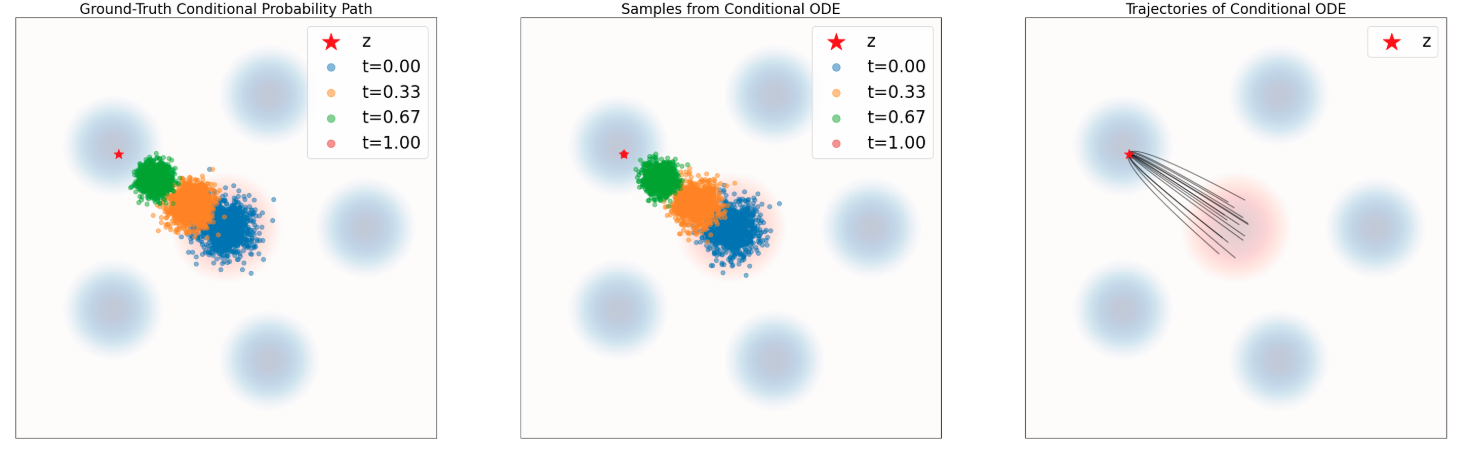
\includegraphics[width=\textwidth]{figures/conditional_ode.png}
   \label{fig:Ng1} 
\end{subfigure}
\begin{subfigure}[b]{\textwidth}
    \centering
   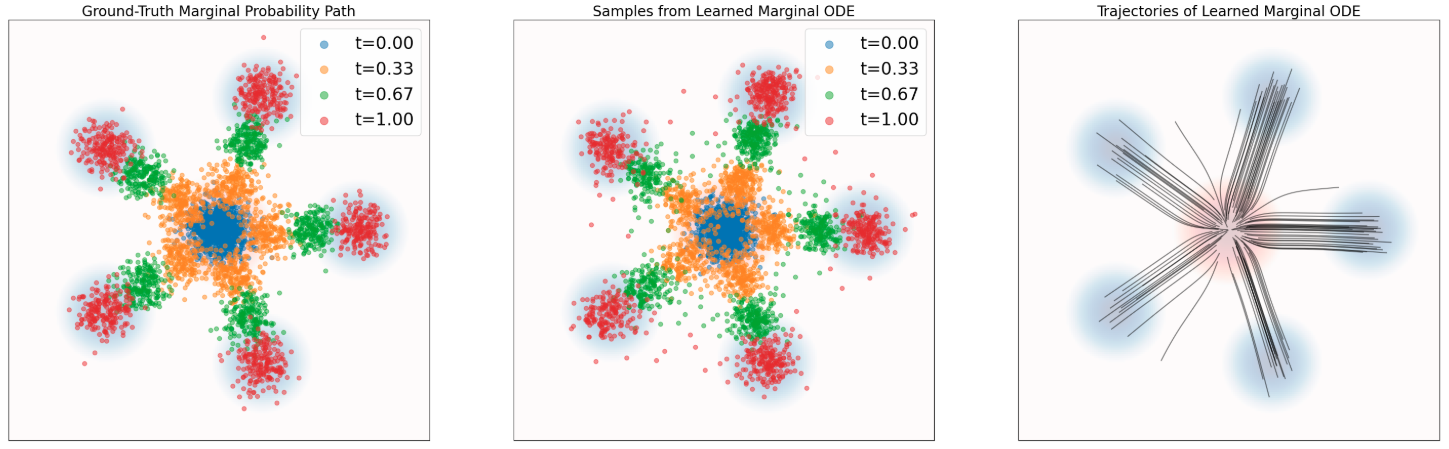
\includegraphics[width=\textwidth]{figures/marginal_ode.png}
   \label{fig:Ng2}
\end{subfigure}
\caption{\label{fig:cond_marginal_path_simulation}Illustration of \cref{thm:marginalization_trick}. Simulating a  probability path with ODEs. Data distribution $\pdata$ in blue background. Gaussian $\pinit$ in red background. Top row: Conditional probability path. Left: Ground truth samples from conditional path $p_t(\cdot|z)$. Middle: ODE samples over time. Right: Trajectories by simulating ODE with $\uref_t(x|z)$ in \cref{eq:conditional_gaussian_vf}. Bottom row: Simulating a marginal probability path. Left: Ground truth samples from $p_t$. Middle: ODE samples over time. Right: Trajectories by simulating ODE with marginal vector field $\uflow_t(x)$. As one can see, the conditional vector field follows the conditional probability path and the marginal vector field follows the marginal probability path. / \cref{thm:marginalization_trick}的图示。使用ODEs模拟概率路径。数据分布$\pdata$为蓝色背景。高斯分布$\pinit$为红色背景。上排:条件概率路径。左:来自条件路径$p_t(\cdot|z)$的真值样本。中:随时间变化的ODE样本。右:通过用\cref{eq:conditional_gaussian_vf}中的$\uref_t(x|z)$模拟ODE得到的轨迹。下排:模拟边际概率路径。左:来自$p_t$的真值样本。中:随时间变化的ODE样本。右:通过用边际向量场$\uflow_t(x)$模拟ODE得到的轨迹。如可以看到,条件向量场遵循条件概率路径,边际向量场遵循边际概率路径。}
\end{figure}
\begin{examplebox}[Target ODE for Gaussian probability paths]
As before, let $p_t(\cdot|\dap) = \mathcal{N}(\alpha_t \dap,\beta_t^2 I_d)$ for noise schedulers $\alpha_t,\beta_t$ (see \cref{eq:gaussian_conditional_probability_paths}). Let $\dot{\alpha}_t=\partial_t\alpha_t$ and $\dot{\beta}_t=\partial_t\beta_t$ denote respective time derivatives of $\alpha_t$ and $\beta_t$. Here, we want to show that the \themebf{conditional Gaussian vector field} given by

如前所述,对于噪声调度器 $\alpha_t,\beta_t$,设 $p_t(\cdot|\dap) = \mathcal{N}(\alpha_t \dap,\beta_t^2 I_d)$(见 \cref{eq:gaussian_conditional_probability_paths})。设 $\dot{\alpha}_t=\partial_t\alpha_t$ 和 $\dot{\beta}_t=\partial_t\beta_t$ 分别表示 $\alpha_t$ 和 $\beta_t$ 的时间导数。在这里,我们想要证明由以下给出的 \themebf{条件高斯向量场}
\begin{align}
\label{eq:conditional_gaussian_vf}
    \uref_t(x|z) = \left(\dot{\alpha}_t-\frac{\dot{\beta}_t}{\beta_t}\alpha_t\right)z+\frac{\dot{\beta}_t}{\beta_t}x
\end{align}
is a valid conditional vector field model in the sense of \cref{thm:marginalization_trick}: its ODE trajectories $X_t$ satisfy $X_t\sim p_t(\cdot|z)=\mathcal{N}(\alpha_t z,\beta_t^2I_d)$ if $X_0\sim \mathcal{N}(0,I_d)$. In \cref{fig:cond_marginal_path_simulation}, we confirm this visually by comparing samples from the conditional probability path (ground truth) to samples from simulated ODE trajectories of this flow. As you can see, the distribution match. We will now prove this.

是 \cref{thm:marginalization_trick} 意义下的有效条件向量场模型:如果 $X_0\sim \mathcal{N}(0,I_d)$,其 ODE 轨迹 $X_t$ 满足 $X_t\sim p_t(\cdot|z)=\mathcal{N}(\alpha_t z,\beta_t^2I_d)$。在 \cref{fig:cond_marginal_path_simulation} 中,我们通过比较条件概率路径的样本(真实值)与该流的模拟 ODE 轨迹样本来视觉确认这一点。如您所见,分布匹配。我们现在将证明这一点。

\begin{proof}
Let us construct a conditional flow model $\psiref_t(x|z)$ first by defining

让我们首先通过定义来构建条件流模型 $\psiref_t(x|z)$
\begin{align}
    \label{eq:cond_flow_gaussian}
    \psiref_t(x|z) = \alpha_t z + \beta_t x.
\end{align}
If $X_t$ is the ODE trajectory of $\psiref_t(\cdot|z)$ with $X_0\sim\pinit = \mathcal{N}(0,I_d)$, then by definition

如果 $X_t$ 是具有 $X_0\sim\pinit = \mathcal{N}(0,I_d)$ 的 $\psiref_t(\cdot|z)$ 的 ODE 轨迹,那么根据定义
\begin{align*}
    X_t = \psiref_t(X_0|z) = \alpha_t z + \beta_t X_0 \sim \mathcal{N}(\alpha_t z,\beta^2 I_d) = p_t(\cdot|z).
\end{align*}
We conclude that the trajectories are distributed like the conditional probability path (i.e, \cref{eq:cond_ref_ode_conds} is fulfilled). It remains to extract the vector field $\uref_t(x|z)$ from $\psiref_t(x|z)$. By the definition of a flow (\cref{e:flow_flow}), it holds

我们得出结论,轨迹的分布与条件概率路径相同(即满足 \cref{eq:cond_ref_ode_conds})。剩下的是从 $\psiref_t(x|z)$ 中提取向量场 $\uref_t(x|z)$。根据流的定义(\cref{e:flow_flow}),有
\begin{align*}
      \frac{\dd}{\dd t}\psiref_{t}(x|z) &= \uref_t(\psiref_t(x|z)|z)\quad \text{ for all }x,z\in\mathbb{R}^d\\
    \overset{(i)}{\Leftrightarrow} \quad \dot{\alpha}_tz+\dot{\beta}_tx &= \uref_t(\alpha_tz+\beta_t x|z)\quad \text{ for all }x,z\in\mathbb{R}^d\\
    \overset{(ii)}{\Leftrightarrow} \quad \dot{\alpha}_tz+\dot{\beta}_t\left(\frac{x-\alpha_tz}{\beta_t}\right)&= \uref_t(x|z)\quad \text{ for all }x,z\in\mathbb{R}^d\\
    \overset{(iii)}{\Leftrightarrow} \quad\left(\dot{\alpha}_t-\frac{\dot{\beta}_t}{\beta_t}\alpha_t\right)z+\frac{\dot{\beta}_t}{\beta_t}x &= \uref_t(x|z)\quad \text{ for all }x,z\in\mathbb{R}^d
\end{align*}
where in $(i)$ we used the definition of $\psiref_t(x|z)$ (\cref{eq:cond_flow_gaussian}), in $(ii)$ we reparameterized $x\rightarrow (x-\alpha_t z)/\beta_t$, and in $(iii)$ we just did some algebra. Note that the last equation is the conditional Gaussian vector field as we defined in \cref{eq:conditional_gaussian_vf}. This proves the statement.\footnote{One can also double check this by plugging it into the continuity equation introduced later in this section.}

其中在 $(i)$ 中我们使用了 $\psiref_t(x|z)$ 的定义(\cref{eq:cond_flow_gaussian}),在 $(ii)$ 中我们重新参数化了 $x\rightarrow (x-\alpha_t z)/\beta_t$,在 $(iii)$ 中我们只是做了一些代数运算。注意最后的方程就是我们在 \cref{eq:conditional_gaussian_vf} 中定义的条件高斯向量场。这证明了该陈述。\footnote{也可以通过将其代入本节后面介绍的连续性方程来验证这一点。}
\end{proof}
\end{examplebox}

The remainder of this section will now prove \cref{thm:marginalization_trick} via the \themebf{continuity equation}, a fundamental result in mathematics and physics. To explain it, we will require the use of the \themebf{divergence} operator $\divv$, which we define as

本节的其余部分现在将通过 \themebf{连续性方程}(数学和物理学中的一个基本结果)来证明 \cref{thm:marginalization_trick}。为了解释它,我们需要使用 \themebf{散度} 算子 $\divv$,定义为
\begin{align}
\label{eq:divergence_laplacian_definition}
    \divv(v_t)(x)=&\sum\limits_{i=1}^{d}\frac{\partial}{\partial x_i}v_t(x)
\end{align}
\begin{theorem}[Continuity Equation]
\label{thm:continuity_equation}
Let us consider an flow model with vector field $\uref_t$ with $X_0\sim\pinit$. Then $X_t\sim p_t$ for all $0\leq t\leq 1$ if and only if

考虑一个具有向量场 $\uref_t$ 和 $X_0\sim\pinit$ 的流模型。那么对于所有 $0\leq t\leq 1$,$X_t\sim p_t$ 当且仅当
\begin{align}
\label{e:continuity_equation}
\partial_t p_t(x)=-\divv (p_t\uref_t)(x)\quad \text{ for all }x\in\R^d, 0\leq t\leq 1,
\end{align}
where $\partial_tp_t(x)= \frac{\dd}{\dd t}p_t(x)$ denotes the time-derivative of $p_t(x)$. Equation \ref{e:continuity_equation} is known as the \themebf{continuity equation}.

其中 $\partial_tp_t(x)= \frac{\dd}{\dd t}p_t(x)$ 表示 $p_t(x)$ 的时间导数。方程 \ref{e:continuity_equation} 被称为 \themebf{连续性方程}。
\end{theorem}
For the mathematically-inclined reader, we present a self-contained proof of the Continuity Equation in \cref{subsec:proof_fokker_planck}. Before we move on, let us try and understand intuitively the continuity equation. The left-hand side $\partial_tp_t(x)$ describes how much the probability $p_t(x)$ at $x$ changes over time. Intuitively, the change should correspond to the net inflow of probability mass. For a flow model, a particle $X_t$ follows along the vector field $\uref_t$. As you might recall from physics, the divergence measures a sort of net outflow from the vector field. Therefore, the negative divergence measures the net inflow. Scaling this by the total probability mass currently residing at $x$, we get that the net $-\divv (p_tu_t)$ measures the total inflow of probability mass. Since probability mass is conserved, the left-hand and right-hand side of the equation should be the same! We now proceed with a proof of the marginalization trick from \cref{thm:marginalization_trick}.

对于数学倾向的读者,我们在 \cref{subsec:proof_fokker_planck} 中提供了连续性方程的自包含证明。在继续之前,让我们尝试直观地理解连续性方程。左侧 $\partial_tp_t(x)$ 描述了 $x$ 处的概率 $p_t(x)$ 随时间的变化量。直观地说,这种变化应该对应于概率质量的净流入。对于流模型,粒子 $X_t$ 沿着向量场 $\uref_t$ 移动。正如您可能从物理学中回忆起的,散度衡量向量场的某种净流出。因此,负散度衡量净流入。将其乘以当前驻留在 $x$ 的总概率质量,我们得到净 $-\divv (p_tu_t)$ 衡量概率质量的总流入。由于概率质量守恒,方程的左侧和右侧应该相同!我们现在继续证明 \cref{thm:marginalization_trick} 中的边际化技巧。
\begin{proof}
By \cref{thm:continuity_equation}, we have to show that the marginal vector field $\uref_t$, as defined as in \cref{eq:marginal_vector_field}, satisfies the continuity equation. We can do this by direct calculation:

根据 \cref{thm:continuity_equation},我们必须证明边际向量场 $\uref_t$(如 \cref{eq:marginal_vector_field} 中定义的)满足连续性方程。我们可以通过直接计算来做到这一点:
\begin{align*}
\partial_t p_t(x) &\overset{(i)}
{=} \partial_t\int p_t(x|\dap) \pdata (z) \dd z\\
&= \int \partial_t p_t(x|\dap) \pdata (z) \dd z\\
&\overset{(ii)}{=} \int -\divv (p_t(\cdot|z)\uref_t(\cdot|z))(x) \pdata (z) \dd z\\
&\overset{(iii)}{=} -\divv \left(\int p_t(x|z) \uref_t(x|z)\pdata(z) \dd z\right)\\
&\overset{(iv)}{=} -\divv \left(p_t(x)\int \uref_t(x|z) \frac{p_t(x|z)\pdata(z)}{p_t(x)}\dd z\right)(x)\\
&\overset{(v)}{=} -\divv \left(p_t\uref_t\right)(x),
\end{align*}
where in $(i)$ we used the definition of $p_t(x)$ in \cref{eq:marginal_prob_path}, in $(ii)$ we used the continuity equation for the conditional probability path $p_t(\cdot|z)$, in $(iii)$ we swapped the integral and divergence operator using \cref{eq:divergence_laplacian_definition}, in $(iv)$ we multiplied and divided by $p_t(x)$, and in $(v)$ we used \cref{eq:marginal_vector_field}. The beginning and end of the above chain of equations show that the continuity equation is fulfilled for $\uref_t$. By \cref{thm:continuity_equation}, this is enough to imply \cref{eq:marginal_ode_follows_marginal_path}, and we are done.

其中在 $(i)$ 中我们使用了 \cref{eq:marginal_prob_path} 中 $p_t(x)$ 的定义,在 $(ii)$ 中我们使用了条件概率路径 $p_t(\cdot|z)$ 的连续性方程,在 $(iii)$ 中我们使用 \cref{eq:divergence_laplacian_definition} 交换了积分和散度算子,在 $(iv)$ 中我们乘除了 $p_t(x)$,在 $(v)$ 中我们使用了 \cref{eq:marginal_vector_field}。上述方程链的开始和结束表明连续性方程对 $\uref_t$ 成立。根据 \cref{thm:continuity_equation},这足以推出 \cref{eq:marginal_ode_follows_marginal_path},我们完成了证明。
\end{proof}


\begin{figure}[t!]
\centering
   \begin{subfigure}[b]{\textwidth}
   \centering
   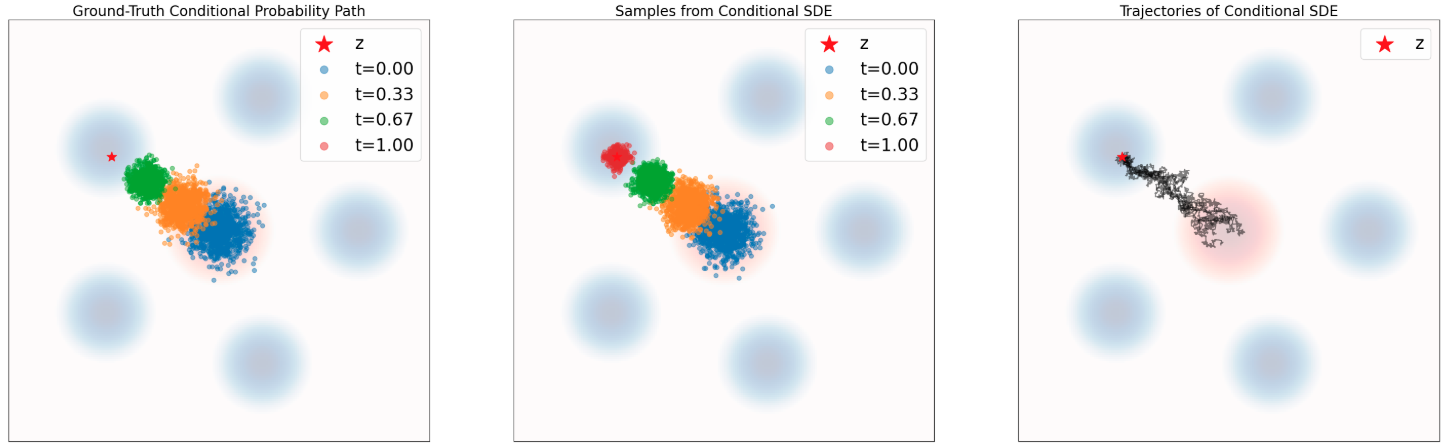
\includegraphics[width=\textwidth]{figures/conditional_sde.png}
   \label{fig:Ng1} 
\end{subfigure}
\begin{subfigure}[b]{\textwidth}
    \centering
   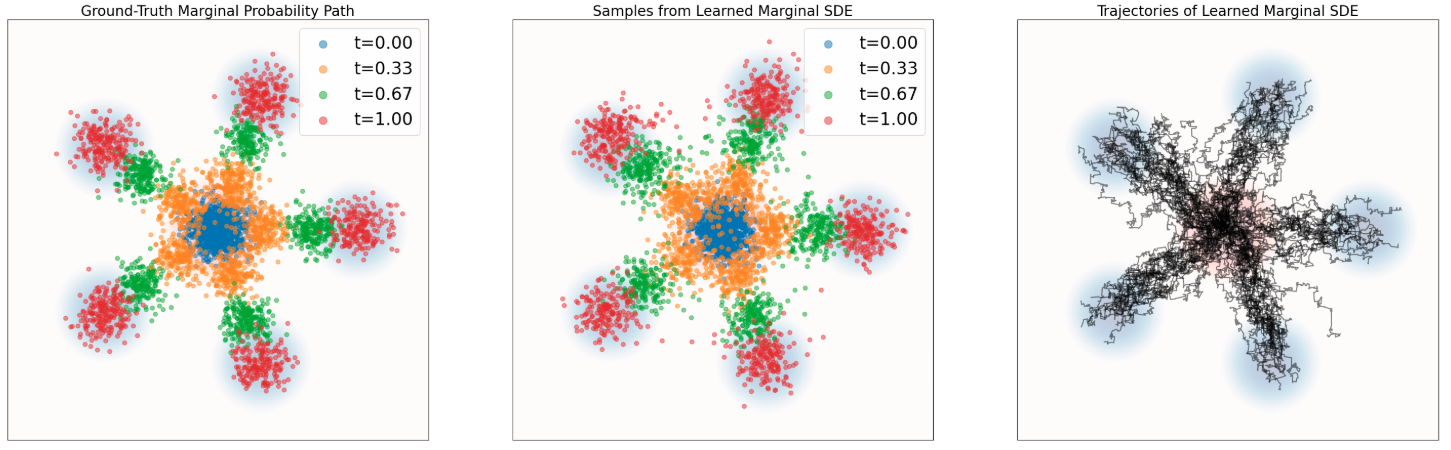
\includegraphics[width=\textwidth]{figures/marginal_sde.png}
   \label{fig:Ng2}
\end{subfigure}
\caption{\label{fig:thm_sde_extension}Illustration of \cref{thm:langevin_trick}. Simulating a probability path with SDEs. This repeats the plots from \cref{fig:cond_marginal_path_simulation} with SDE sampling using \cref{eq:sde_extension}. Data distribution $\pdata$ in blue background. Gaussian $\pinit$ in red background. Top row: Conditional path. Bottom row: Marginal probability path. As one can see, the SDE transports samples from $\pinit$ into samples from $\delta_{z}$ (for the conditional path) and to $\pdata$ (for the marginal path). / \cref{thm:langevin_trick}的图示。使用SDEs模拟概率路径。这重复了\cref{fig:cond_marginal_path_simulation}中的图,使用\cref{eq:sde_extension}进行SDE采样。数据分布$\pdata$为蓝色背景。高斯分布$\pinit$为红色背景。上排:条件路径。下排:边际概率路径。如可以看到,SDE将样本从$\pinit$传输到$\delta_{z}$的样本(对于条件路径)和$\pdata$(对于边际路径)。}
\end{figure}

\subsection{Conditional and Marginal Score Functions}

We just successfully constructed a training target for a flow model. We now extend this reasoning to SDEs. To do so, let us define the \themebf{marginal score function} of $p_t$ as $\nabla\log p_t(x)$. We can use this to extend the ODE from the previous section to an SDE, as the following result demonstrates.

我们刚刚成功构建了流模型的训练目标。现在我们将这种推理扩展到 SDE。为此,让我们将 $p_t$ 的 \themebf{边际得分函数} 定义为 $\nabla\log p_t(x)$。我们可以使用它将上一节的 ODE 扩展到 SDE,如下面的结果所示。
\begin{theorem}[SDE extension trick]
\label{thm:langevin_trick}
Define the conditional and marginal vector fields $\uref_t(x|z)$ and $\uref_t(x)$ as before. Then, for diffusion coefficient $\sigma_t\geq 0$, we may construct an SDE which follows the same probability path:

如前所述定义条件和边际向量场 $\uref_t(x|z)$ 和 $\uref_t(x)$。那么,对于扩散系数 $\sigma_t\geq 0$,我们可以构建一个遵循相同概率路径的 SDE:
\begin{align}
\label{eq:sde_extension}
    X_0\sim&\pinit,\quad \dd X_t =\left[\uref_t(X_t)+\frac{\sigma_t^2}{2}\nabla\log p_t(X_t)\right]\dd t +\sigma_t\dd W_t\\
    \label{eq:marginal_ode_follows_marginal_path_sde}
    \Rightarrow X_t\sim& p_t\quad (0\leq t\leq 1)
\end{align}
In particular, $X_1\sim \pdata$ for this SDE. The same identity holds if we replace the marginal probability $p_t(x)$ and vector field $\uref_t(x)$ with the conditional probability path $p_t(x|z)$ and vector field $\uref_t(x|z)$.

特别地,对于这个SDE,$X_1\sim \pdata$。如果我们用条件概率路径$p_t(x|z)$和向量场$\uref_t(x|z)$分别替换边际概率$p_t(x)$和向量场$\uref_t(x)$,同样的恒等式也成立。
\end{theorem}
We illustrate the theorem in \cref{fig:thm_sde_extension}. The formula in \cref{thm:langevin_trick} is useful because, similar to before, we can express the marginal score function via the \themebf{conditional score function} $\nabla\log p_t(x|z)$

我们在 \cref{fig:thm_sde_extension} 中说明了这个定理。\cref{thm:langevin_trick} 中的公式是有用的,因为与之前类似,我们可以通过 \themebf{条件得分函数} $\nabla\log p_t(x|z)$ 来表达边际得分函数
\begin{align}
\label{e:marginal_score}
\nabla\log p_t(x) = \frac{\nabla p_t(x)}{p_t(x)}
=\frac{\nabla \int p_t(x|z)\pdata(z)\dd z}{p_t(x)}
=\frac{\int \nabla p_t(x|z)\pdata(z)\dd z}{p_t(x)}
=\int \nabla \log p_t(x|z)\frac{ p_t(x|z)\pdata(z)}{p_t(x)}\dd z
\end{align}
and the conditional score function $\nabla \log p_t(x|z)$ is something we usually know analytically, as illustrated by the following example.

条件得分函数 $\nabla \log p_t(x|z)$ 通常是我们可以解析获得的,如下面的例子所示。
\begin{examplebox}[Score Function for Gaussian Probability Paths.] 
For the Gaussian path $p_t(x|z)=\mathcal{N}(x;\alpha_t z,\beta_t^2 I_d)$, we can use the form of the Gaussian probability density (see \cref{e:gaussian}) to get

对于高斯路径 $p_t(x|z)=\mathcal{N}(x;\alpha_t z,\beta_t^2 I_d)$,我们可以使用高斯概率密度的形式(见 \cref{e:gaussian})来得到

\begin{align}
\label{eq:cond_score_gaussian}
    \nabla \log p_t(x|z) = \nabla\log \mathcal{N}(x;\alpha_t z,\beta_t^2 I_d) = -\frac{x-\alpha_t z}{\beta_t^2}.
\end{align}

Note that the score is a linear function of $x$. This is a unique feature of Gaussian distributions.

注意,得分函数是 $x$ 的线性函数。这是高斯分布的一个独特特征。
\end{examplebox}

在本节的其余部分,我们将通过 \themebf{福克-普朗克方程} 来证明 \cref{thm:langevin_trick},该方程将连续性方程从 ODE 扩展到 SDE。为此,让我们首先通过以下方式定义 \themebf{拉普拉斯} 算子 $\Delta$
\begin{align}
    \label{eq:laplacian_definition}
    \Delta w_t(x)=&\sum\limits_{i=1}^{d}\frac{\partial^2}{\partial^2 x_i}w_t(x)=\divv(\nabla w_t)(x).
\end{align}
\begin{theorem}[Fokker-Planck Equation]
\label{thm:fokker_planck}
Let $p_t$ be a probability path and let us consider the SDE

设 $p_t$ 是一个概率路径,考虑 SDE
\begin{align*}
    X_0\sim \pinit, \quad \dd X_t = u_t(X_t)\dd t + \sigma_t\dd W_t.
\end{align*}
Then $X_t$ has distribution $p_t$ for all $0\leq t\leq 1$ if and only if the \themebf{Fokker-Planck equation} holds:

那么对于所有 $0\leq t\leq 1$,$X_t$ 具有分布 $p_t$ 当且仅当 \themebf{福克-普朗克方程} 成立:
    \begin{align}
    \label{e:fokker_planck}
    \partial_t p_t(x) = -\divv (p_t u_t)(x)+\frac{\sigma_t^2}{2}\Delta p_t (x)\quad \text{ for all }x\in\R^d, 0\leq t\leq 1.
    \end{align}     
\end{theorem}
A self-contained proof of the Fokker-Planck equation can be found in \cref{subsec:proof_fokker_planck}. Note that the continuity equation is recovered from the Fokker-Planck equation when $\sigma_t=0$. The additional Laplacian term $\Delta p_t$ might be hard to rationalize at first. Those familiar with physics will note that the same term also appears in the heat equation (which is in fact a special case of the Fokker-Planck equation). Heat diffuses through a medium. We also add a diffusion process (not a physical but a mathematical one) and hence we add this additional Laplacian term. 

福克-普朗克方程的自包含证明可在 \cref{subsec:proof_fokker_planck} 中找到。注意当 $\sigma_t=0$ 时,连续性方程可以从福克-普朗克方程中恢复。额外的拉普拉斯项 $\Delta p_t$ 起初可能难以理解。那些熟悉物理学的人会注意到,同样的项也出现在热方程中(实际上是福克-普朗克方程的特例)。热量在介质中扩散。我们也添加了一个扩散过程(不是物理的而是数学的),因此我们添加了这个额外的拉普拉斯项。

Let us now use the Fokker-Planck equation to help us prove \cref{thm:langevin_trick}.

现在让我们使用福克-普朗克方程来帮助证明 \cref{thm:langevin_trick}。

\begin{proof}[Proof of \Cref{thm:langevin_trick}]
 By \cref{thm:fokker_planck}, we need to show that that the SDE defined in \cref{eq:sde_extension} satisfies the Fokker-Planck equation for $p_t$. We can do this by direction calculation:

根据 \cref{thm:fokker_planck},我们需要证明 \cref{eq:sde_extension} 中定义的 SDE 满足 $p_t$ 的福克-普朗克方程。我们可以通过直接计算来做到这一点:
\begin{align*}
    \partial_t p_t(x) \overset{(i)}{=}& - \divv(p_t\uref_t)(x)\\
    \overset{(ii)}{=}& - \divv(p_t\uref_t)(x) -\frac{\sigma_t^2}{2}\Delta p_t(x)+\frac{\sigma_t^2}{2}\Delta p_t(x)\\
    \overset{(iii)}{=}& - \divv(p_t\uref_t)(x) -\divv(\frac{\sigma_t^2}{2}\nabla p_t)(x)+\frac{\sigma_t^2}{2}\Delta p_t(x)\\
    \overset{(iv)}{=}& - \divv(p_t\uref_t)(x) -\divv(p_t\left[\frac{\sigma_t^2}{2}\nabla \log p_t\right])(x)+\frac{\sigma_t^2}{2}\Delta p_t(x)\\
    \overset{(v)}{=}&- \divv\left(p_t\left[\uref_t+\frac{\sigma_t^2}{2}\nabla \log p_t\right]\right)(x)+\frac{\sigma_t^2}{2}\Delta p_t(x),
\end{align*}
where in $(i)$ we used the Contuity Equation, in $(ii)$ we added and subtracted the same term, in $(iii)$ we used the definition of the Laplacian (\cref{eq:laplacian_definition}), in $(iv)$ we used that $\nabla\log p_t=\frac{\nabla p_t}{p_t}$, and in $(v)$ we used the linearity of the divergence operator. The above derivation shows that the SDE defined in \cref{eq:sde_extension} satisfies the Fokker-Planck equation for $p_t$. By \cref{thm:fokker_planck}, this implies $X_t\sim p_t$ for $0\leq t\leq 1$, as desired.

其中在 $(i)$ 中我们使用了连续性方程,在 $(ii)$ 中我们加减了同一项,在 $(iii)$ 中我们使用了拉普拉斯算子的定义(\cref{eq:laplacian_definition}),在 $(iv)$ 中我们使用了 $\nabla\log p_t=\frac{\nabla p_t}{p_t}$,在 $(v)$ 中我们使用了散度算子的线性性。上述推导表明 \cref{eq:sde_extension} 中定义的 SDE 满足 $p_t$ 的福克-普朗克方程。根据 \cref{thm:fokker_planck},这意味着对于 $0\leq t\leq 1$,有 $X_t\sim p_t$,正如所期望的。
\end{proof}

\begin{figure}[!t]
    \centering
    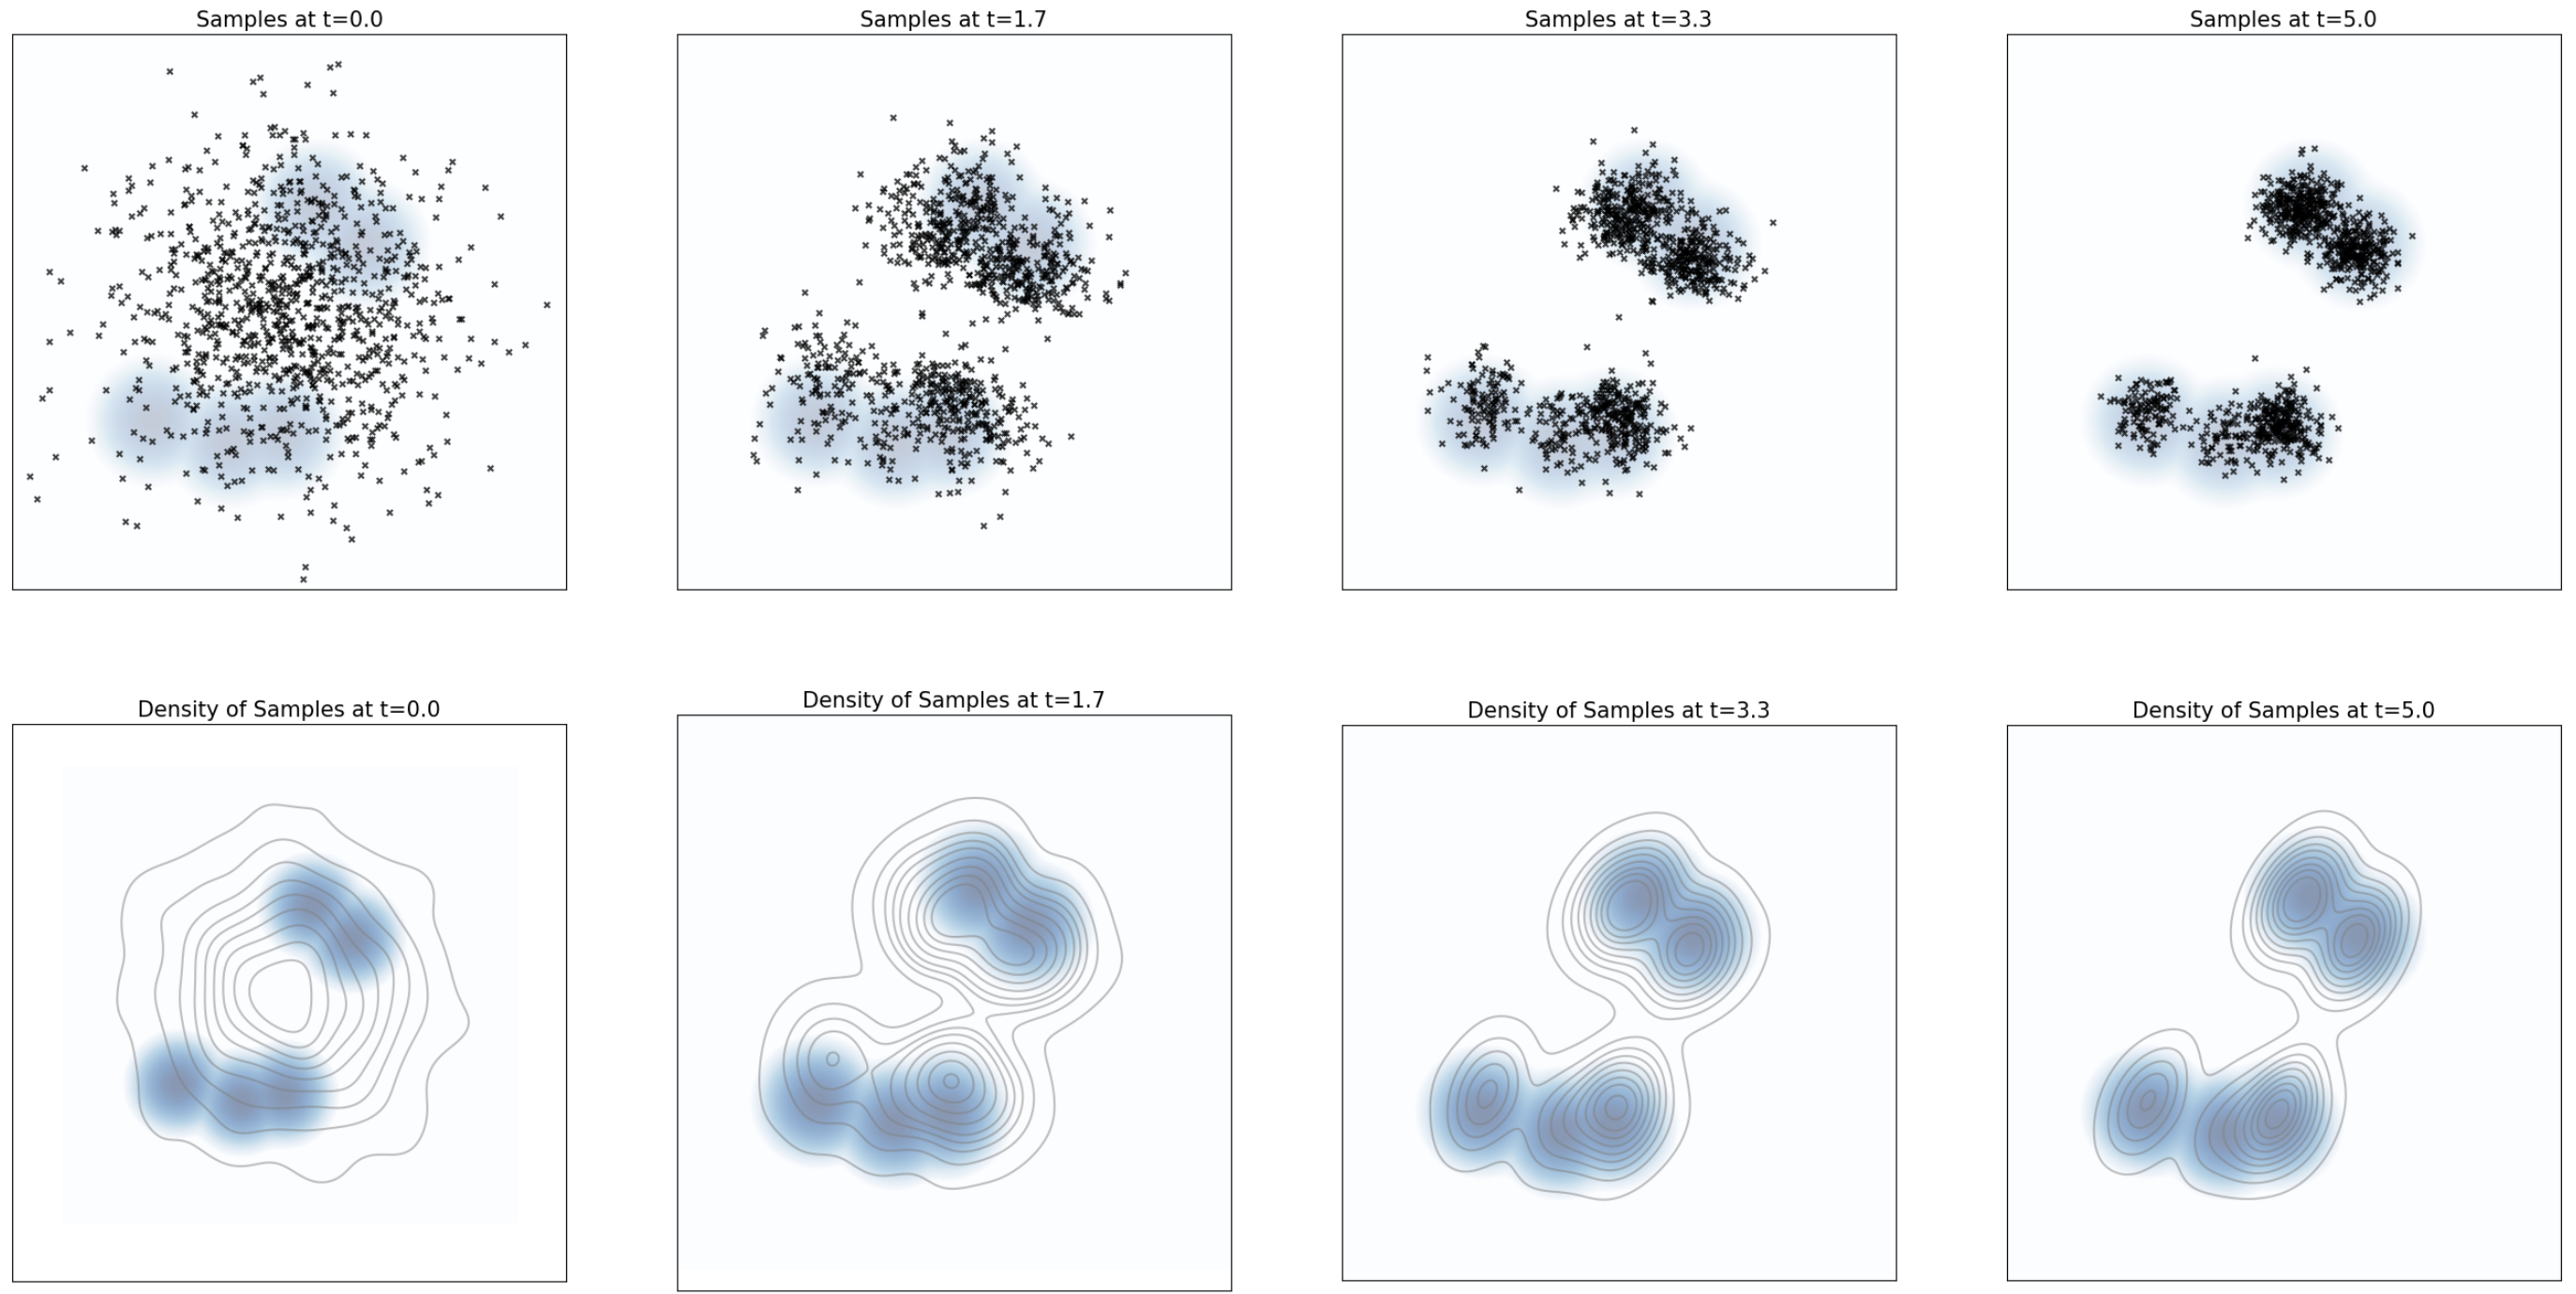
\includegraphics[width=\textwidth]{figures/langevin.png}
    \label{fig:langevin}
    \caption{
        Top row: Particles evolving under the Langevin dynamics given by \cref{eq:langevin_dynamics}, with $p(x)$ taken to be a Gaussian mixture with 5 modes. 
        Bottom row: A kernel density estimate of the same samples shown in the top row. 
        As one can see, the distribution of samples converges to the equilibrium distribution $p$ (blue background colour).
        第一行:粒子在 \cref{eq:langevin_dynamics} 给出的朗之万动力学下演化,其中 $p(x)$ 被取为具有 5 个模式的高斯混合。
        第二行:第一行所示相同样本的核密度估计。如您所见,样本的分布收敛到平衡分布 $p$(蓝色背景色)。
    } 
\end{figure}
\begin{remarkbox}[Langevin dynamics.]
The above construction has a famous special case when the probability path is static, i.e. $p_t=p$ for a fixed distribution $p$. In this case, we set $\uref_t=0$ and obtain the SDE

上述构造有一个著名的特殊情况,即当概率路径是静态的时,即对于固定分布 $p$ 有 $p_t=p$。在这种情况下,我们设置 $\uref_t=0$ 并得到 SDE

\begin{equation}
    \dd X_t = \frac{\sigma_t^2}{2}\nabla\log p(X_t)\dd t + \sigma_t dW_t \label{eq:langevin_dynamics},
\end{equation}

which is commonly known as \themebf{Langevin dynamics}. The fact that $p_t$ is static implies that $\partial_tp_t(x)=0$. It follows immediately from \cref{thm:langevin_trick} that these dynamics satisfy the Fokker-Planck equation for the static path $p_t=p$ in \cref{thm:langevin_trick}. Therefore, we may conclude that $p$ is a stationary distribution of Langevin dynamics, so that

这通常被称为\themebf{朗之万动力学}。$p_t$ 是静态的这一事实意味着 $\partial_tp_t(x)=0$。从 \cref{thm:langevin_trick} 立即可知,这些动力学满足 \cref{thm:langevin_trick} 中静态路径 $p_t=p$ 的福克-普朗克方程。因此,我们可以得出结论,$p$ 是朗之万动力学的平稳分布,使得

\begin{align*}
    X_0 \sim p\quad \Rightarrow \quad X_t \sim p\quad (t\geq 0)
\end{align*}

As with many Markov chains, these dynamics converge to the stationary distribution $p$ under rather general conditions (see \cref{fig:langevin}). That is, if we instead we take $X_0 \sim p' \neq p$, so that $X_t \sim p_t'$, then under mild conditions $p_t \to p$. This fact makes Langevin dynamics extremely useful, and it accordingly serves as the basis for e.g., \textbf{molecular dynamics} simulations, and many other Markov chain Monte Carlo (MCMC) methods across Bayesian statistics and the natural sciences.

与许多马尔可夫链一样,这些动力学在相当一般的条件下会收敛到平稳分布 $p$(见 \cref{fig:langevin})。也就是说,如果我们取 $X_0 \sim p' \neq p$,使得 $X_t \sim p_t'$,那么在温和条件下 $p_t \to p$。这一事实使得朗之万动力学极其有用,因此它作为例如\textbf{分子动力学}模拟以及贝叶斯统计和自然科学中许多其他马尔可夫链蒙特卡罗(MCMC)方法的基础。
\end{remarkbox}

Let us summarize the results of this section.

让我们总结本节的结果。
\begin{summarybox}[Derivation of the Training Target]
\textbf{The flow training target is the marginal vector field $\uref_t$.} To construct it, we choose a \themebf{conditional probability path} $p_t(x|\dap)$ that fulfils $p_0(\cdot|z)=\pinit$, $p_1(\cdot|z)=\delta_{z}$. Next, we find a \themebf{conditional vector field} $\uflow_t(x|z)$ such that its corresponding flow $\psiref_t(x|z)$ fulfills

\textbf{流模型的训练目标是边际向量场 $\uref_t$。} 为了构建它,我们选择一个满足 $p_0(\cdot|z)=\pinit$, $p_1(\cdot|z)=\delta_{z}$ 的 \themebf{条件概率路径} $p_t(x|\dap)$。接下来,我们找到一个 \themebf{条件向量场} $\uflow_t(x|z)$,使得其对应的流 $\psiref_t(x|z)$ 满足
\begin{align*}
    X_0\sim \pinit \quad \Rightarrow \quad X_t = \psiref_t(X_0|z) \sim p_t(\cdot|z),
\end{align*}
or, equivalently, that $\uref_t$ satisfies the continuity equation.  Then the \themebf{marginal vector field} defined by

或者等价地,$\uref_t$ 满足连续性方程。然后由以下定义的 \themebf{边际向量场}
\begin{align}
    \label{eq:marginal_vector_field_restated}
    \uref_t(x) = \int \uref_t(x|z)\frac{p_t(x|z)\pdata(z)}{p_t(x)}\dd z,
\end{align}
follows the marginal probability path, i.e.,

遵循边际概率路径,即
\begin{align}
    \label{eq:marginal_ode_follows_marginal_path_restated}
    X_0&\sim\pinit,\quad \dd X_t =\uref_t(X_t)\dd t\Rightarrow X_t\sim p_t\quad (0\leq t\leq 1).
\end{align}
In particular, $X_1\sim \pdata$ for this ODE, so that $\uref_t$ "converts noise into data", as desired.

特别地,对于这个 ODE,有 $X_1\sim \pdata$,因此 $\uref_t$ "将噪声转换为数据",正如所期望的。


\textbf{Extending to SDEs.} For a time-dependent diffusion coefficient $\sigma_t\geq 0$, we can extend the above ODE to an SDE with the same marginal probability path:

\textbf{扩展到 SDE。} 对于时间相关的扩散系数 $\sigma_t\geq 0$,我们可以将上述 ODE 扩展为具有相同边际概率路径的 SDE:
\begin{align}
\label{eq:sde_extension_restated}
    X_0\sim&\pinit,\quad \dd X_t =\left[\uref_t(X_t)+\frac{\sigma_t^2}{2}\nabla\log p_t(X_t)\right]\dd t +\sigma_t\dd W_t\\
    \label{eq:marginal_ode_follows_marginal_path_restated}
    \Rightarrow X_t\sim& p_t\quad (0\leq t\leq 1),
\end{align}
where $\nabla\log p_t(x)$ is the \themebf{marginal score function}

其中 $\nabla\log p_t(x)$ 是 \themebf{边际得分函数}
\begin{align}
\nabla\log p_t(x) =&\int \nabla \log p_t(x|z)\frac{ p_t(x|z)\pdata(z)}{p_t(x)}\dd z.
\end{align}
In particular, for the trajectories $X_t$ of the above SDE, it holds that $X_1\sim \pdata$, so that the SDE "converts noise into data", as desired. An important example is the \themebf{Gaussian probability path}, yielding the formulae:

特别地,对于上述 SDE 的轨迹 $X_t$,有 $X_1\sim \pdata$,因此 SDE "将噪声转换为数据",正如所期望的。一个重要的例子是 \themebf{高斯概率路径},产生以下公式:
\begin{align}
p_t(x|z) =& \mathcal{N}(x;\alpha_t z,\beta_t^2 I_d)\\
\uflow_t(x|z)=&\left(\dot{\alpha}_t-\frac{\dot{\beta}_t}{\beta_t}\alpha_t\right)z+\frac{\dot{\beta}_t}{\beta_t}x\\
\nabla \log p_t(x|z) =& -\frac{x-\alpha_t z}{\beta_t^2},
\end{align}
for \themebf{noise schedulers} $\alpha_t,\beta_t\in\mathbb{R}$: continuously differentiable, monotonic functions such that $\alpha_0=\beta_1=0$ $\alpha_1=\beta_0=1$.

对于 \themebf{噪声调度器} $\alpha_t,\beta_t\in\mathbb{R}$:连续可微的单调函数,满足 $\alpha_0=\beta_1=0$,$\alpha_1=\beta_0=1$。
\end{summarybox}

% \subsection{Optimizing over all possible reference diffusion models.}\mycomment{Neural ODEs, Schrödinger Bridges.}
% % Note that the condition in \cref{e:reference_sde_condition} does not say anything about distributions $X_t\sim p_t^$ at intermediate time points $0<t<1$ - we only require the initial distribution at $t=0$ to be 
% % $\pinit$ and the final distribution to be $\pdata$ at $t=1$. Therefore, there is more degrees of freedom that we are allowed to choose.
% \label{e:reference_sde_condition} 
% our goal in \cref{e:end_points_match} doesn't say anything about how $p_t^\theta$ should look like for intermediate time points $0<t<1$
